%! TEX root = ../barycenter.tex
\YYCleverefInput{/var/tmp/latex/barycenter.sed}
\subsection{Absolutely continuity in general case}

In general case, we shall find relations between density functions.
This involves Jacobian of push-forward maps,
and thus we need to study Hessian of $c$-concave functions.

\subsubsection{Hessian almost everywhere}

In this subsection, we aim to give a proper definition of Hessian
for $c$-concave function
though its first order differential is not defined everywhere.
As $c$-concave function has always super-differential, we give a corresponding
definition of Hessian using super-differential.

\begin{defn}[Hessian]
	Let \( \phi : \Omega \rightarrow \mathbb { R } \) be
	a	super-differentiable function
	on an open set \( \Omega \subset M \)
	We say that \( \phi \) has \( a \) Hessian \( H \) at \( x \in \Omega \) if \( \phi \) is differentiable at \( x \)
	and there exists a self-adjoint operator \( H : T _ { x } M \rightarrow T _ { x } M \) satisfying
	\begin{equation}
		\label{defn:hessian}
		\sup _ { v \in \partial \phi \left( \exp _ { x } u \right) } \left| \Pi _ { x , u } v - \nabla \phi ( x ) - H u \right| = o ( | u | )
	\end{equation}
	as \( u \rightarrow 0 \) in \( T _ { x } M \). Here \( \Pi _ { x , u } : T _ { \exp _ { x } u } M \rightarrow T _ { x } M \) denotes parallel translation to \( x \) along \( \gamma ( t ) : = \exp _ { x } ( t u ) . \) The Hessian of \( \phi \) at \( x \) may also be denoted
	by \( \operatorname { Hess } _ { x } \phi : = H \).
\end{defn}

This definition coincides with the usual one for smooth functions. A more intuitive understanding of the Hessian follows from the fact that existence of a Hessian \( H \) at \( x \) for \( \phi \) implies a second order Taylor expansion for \( \phi \) around \( x : \) as \( u \rightarrow 0 \in T _ { x } M \),
\begin{equation}
	\label{equa:hessian_expan}
	\phi \left( \exp _ { x } u \right) = \phi ( x ) + \langle \nabla \phi ( x ) , u \rangle + \frac { 1 } { 2 } \langle H u , u \rangle + o \left( | u | ^ { 2 } \right).
\end{equation}

Following theorem (\cite[Proposition 3.4]{cordero2001riemannian}) justifies the usage of word ``concave''.
\begin{thm}[$c$-concave function has Hessian almost everywhere]
	\label{thm:c-concave_hessain}
	Let $\mathcal{X} \subset \subset M$ be open and $Y \subset M$ be compact.
	Every $c$-concave function in $\mathcal{I}^c(\bar { \mathcal{X}}, Y )$ has Hessian
	almost everywhere with respect to the volume measure on $M$.
\end{thm}

\begin{prop} [Differentiating optimal transport]
	\label{prop:differentiate_optimal_transport}
	Fix \( \mathcal{X} \subset \subset M \) be open and \( Y \subset M \) compact.
	Let \( \phi \in \mathcal{I} ^ { c } ( \bar { \mathcal{X} } , Y ) \) and set \( F ( z ) : = \exp _ { z } ( - \nabla \phi ( z ) ) . \)
	Fix a point \( x \in \mathcal{X} \) where \( \phi \) admits a Hessian \cref{defn:hessian}.
	Then:
	\begin{enumerate}
		\item \( y : = F ( x ) \notin \operatorname { cut } ( x ) \) and setting \( H : = \operatorname { Hess } _ { x } d _ { y } ^ { 2 } / 2 \), one has \( H - \operatorname { Hess } _ { x } \phi \) \( \geq 0 \)
		\item Introduce \( Y : = \diff \left( \exp _ { x } \right) _ { - \nabla \phi ( x ) } \) and define \( \diff F _ { x } : T _ { x } M \rightarrow T _ { y } M \) by
		      \( \diff F _ { x } : = Y \left( H - \operatorname { Hess } _ { x } \phi \right) \).
		      Then as \( u \rightarrow 0 \) in \( T _ { x } M \),
		      \begin{equation}
			      \label{equa:differentiate_optimal_transport}
			      \sup _ {\substack {\exp _ { y } v \in \partial ^ { c } \phi \left( \exp _ { x } u \right) \\
					      | v | = d \left( y , \exp _ { y } v \right)} } \left| v - \diff F _ { x } ( u ) \right| = o ( | u | )
		      \end{equation}

	\end{enumerate}
\end{prop}

It helps to mention that by \cref{example:minimizer_differentiable} we have
$\partial^c \phi (x) = \{ F(x) \}$.
Then the cryptic \cref{equa:differentiate_optimal_transport} means that we are differentiating
the set value map $z \mapsto \partial^c \phi(z)$.
As $c$-super-differential gives rise to a super-differential by \cref{lem:c-super-gradients_imply_super-gradients},
it makes sense to compare the differential $\diff F_x$ with all super-differential $v$.
\begin{rmk}[Sketch proof for the second point of \cref{prop:differentiate_optimal_transport}]
	% For the first point, we apply the characterization of cut locus in \cref{prop:distance_cut_locus};
	% existence of Hessian for $\phi$ and \cref{equa:c-concave_conjugate} then gives a lower bound for squared distance function $d_y^2$.

	% 	As for the second point,
	It is a clever application of chain rule and \cref{equa:exponential_map_and_squared_distance_function}.
	Ignore the problem of second differentiability for a while, we define
	\[
		g(u,v) = \exp_{u}(-\nabla d_y^2(u) + \nabla d_y^2(v) - \nabla \phi (v)),
	\]
	then $F(z) = g(z, z)$ and $ y = g(u, x) $ is a constant $y = F(x)$.
	This gives that
	\[
		\diff F(x) = \partial_u g(x, x) + \partial_v g(x, x) = \partial_v g(x, x) = Y(H - \operatorname{Hess}_x \phi).
	\]
	A full proof is in \cite[Proposition 4.1]{cordero2001riemannian}.
\end{rmk}

This definition gives Jacobian identity (\cite[Theorem 4.2]{cordero2001riemannian}).

\begin{thm}
	[Jacobian identity a.e.]
	\label{thm:jacobian_identity}
	Let \( \mu \ll \operatorname{Vol} \) and \( \nu \ll \operatorname{Vol} \) be
	two compactly supported Borel probability measures and denote their
	\( L ^ { 1 } ( M, \operatorname{Vol}) \) densities by \( f \) and \( g \), respectively.
	Fix domains \( \mathcal{X} \subset \subset M \) and \( \mathcal{Y} \subset \subset M \) containing the support of \( \mu \) and \( v \), respectively.
	Suppose \( \phi \in \mathcal{I} ^ { c } ( \bar { \mathcal{X} } , \bar { \mathcal{Y} } ) \) induces
	\( F : \mathcal{X} \rightarrow \bar { \mathcal{Y} } \) defined by \( F ( x ) : = \exp _ { x } ( - \nabla \phi ( x ) ) \)
	which pushes \( \mu \) forward to $\nu$.
	Then there exists a Borel set \( K \subset \mathcal{X} \) of full
	measure for \( \mu \) such that
	\begin{enumerate}
		\item $\phi$ admits a Hessian \( \operatorname { Hess } _ { x } \phi \) at each \( x \in K \), and hence \( F ( x ) \notin \operatorname { cut } ( x ) \).
		\item For \( x \in K \), setting \( Y : = \diff \left( \exp _ { x } \right) _ { - \nabla \phi ( x ) } \) and \( H : = \operatorname { Hess } _ { x } d _ { F ( x ) } ^ { 2 } / 2 \), one
		      has
		      \[ f ( x ) = g ( F ( x ) ) \operatorname { det } \left[ Y \left( H - \operatorname { Hess } _ { x } \phi \right) \right] \neq 0 \]
	\end{enumerate}
\end{thm}

We remark that in the proof of this theorem,
it is shown (\cite[Claim 4.3 and Claim 4.4]{cordero2001riemannian}) that
$\det \diff F_x > 0$ holds for $\mu$ almost everywhere.
% And in general $ \det \diff F_x \geq 0$ holds (\cite[Lemma 2.1]{cordero2001riemannian})
% whenever it exists.

\subsubsection{Bound Jacobian by sectional curvature}

There are two terms to bound in the Jacobian $\det[ Y(H - \operatorname{Hess}_x \varphi)]$, $Y$ and $H$;
while we shall eliminate the Hessian of $\varphi$ at the end.
% We bound them using Ricci curvature and
% we can prove these bounds using similar compassion arguments involving Jacobi field.
% We define
% \begin{equation}
% 	S _ { K } ( d ) = \left\{
% 	\begin{array} { l l } \frac { \sin ( \sqrt { K } d ) } { \sqrt { K } d } & \text { if } K > 0 \\
%               1                                                          & \text { if } K = 0
%               \\ \frac { \sinh ( \sqrt { - K } d ) } { \sqrt { - K } d } & \text { if } K < 0
% 	\end{array} \right.
% \end{equation}

Rauch theorem gives bound on $Y$ through section curvature, see
\cite[Theorem IX.2.3]{chavel2006riemannian} for a proof using Jacobi filed.
\begin{prop} [The geometric Rauch theorem]
	Let $\xi$ be unit tangent vector in $T_p M$
	and $\gamma$ a geodesic starting at $p \in M$ with initial speed $\xi$.
	Suppose \( - k < 0 \) is a lower bound for
	the sectional curvatures at every point of \( \gamma \).
	Assume that \( \gamma (t)\) is not in the cut locus of $p$.
	% has no points conjugate to \( p \) along \( \gamma \mid_{( 0 , t ]} \).
	Then, for all \( v \in \xi ^ { \perp } \),
	\begin{equation*}
		% \frac { \mathbf { S } _ { \delta } ( t ) } { t } \leq
		\frac { \left| \diff ( \exp _ { p })  _ {t \xi } \,
			\mathfrak{J}_{t \xi}( v )\right| } { | v | }
		\leq \frac { \sinh (\sqrt{ -k } t )} {\sqrt{-k} t },
	\end{equation*}
	where $\mathfrak{J}_{t \xi}: T_p M \rightarrow T_{t \xi} T_p M$ is the canonical identification
	between two them.
\end{prop}

Following bound (\cite[Lemma 3.12]{cordero2001riemannian}) on $H$ is proved using similar argument.
\begin{prop}[Hessian bound for distance squared]
	\label{lem:hessian_bound_distance_squared}
	Fix \(  x , y \in M \) and
	a minimal geodesic \( \gamma \) joining \( x \) to \( y \).
	Suppose \( - k < 0 \) is a lower bound for
	the sectional curvatures at every point of \( \gamma \).
	Each \( u \in T _ { x } M \) satisfies
	\begin{equation*}
		\label{equa:hessian_bound_distance_squared}
		\limsup _ { r \rightarrow 0 } \frac { d _ { y } ^ { 2 } \left( \exp _ { x } r u \right) + d _ { y } ^ { 2 } \left( \exp _ { x } - r u \right) - 2 d _ { y } ^ { 2 } ( x ) }
		{ r ^ { 2 } } \leq 2 \frac{ \sqrt { k } d ( x , y ) }
		{\tanh ( \sqrt { k } d ( x , y ) )}
	\end{equation*}
\end{prop}
% As observed in \cite[Lemma 2.7]{KIM2017640}, with the same proof as \cite[Lemma 3.12]{cordero2001riemannian},
% we can concatenate sectional curvature to get conclusion in Ricci curvature.
% \begin{lem}
% 	Suppose \( - K \leq 0 \) is a lower bound for the Ricci curvature on \( M \).
% 	Then
% 	\[
% 		\operatorname { tr } \left[ \operatorname{Hess}_x d^ { 2 }_y ( x ) \right]
% 		\leq n \frac { \sqrt { K } d ( x , y ) }
% 		{ \tanh ( \sqrt { K } d ( x , y ) ) } .
% 	\]
% \end{lem}

The right-hand sides of these two bounds are not bounded functions of distance,
thus we must bound the distance in advance.
We do this later by restricting two endpoints of geodesics into two compact sets.
% In the context of \cref{thm:jacobian_identity},
% we fix $ \mathcal{X}, \mathcal{Y} \subset \subset M$ and consider $ \phi \in \mathcal{I} ^c (\bar{ \mathcal{X} }, \bar{ \mathcal{Y} })$,
% then both sectional curvature and distance are bounded by compactness
% ( see the same argument in \cite[Corollary 3.3.7]{cordero2001riemannian});
% so we can bound all eigenvalues for $Y$ and $H$ for function $F: =\exp(- \nabla \phi)$.
% On other hand, we can also impose sectional curvature condition globally.

\subsubsection{Discussion on absolutely continuity by consistency}

Let $\mu_i \in \mathcal{W}_2(M), 1 \leq i \leq n $ be $n$ measures with compact supports.
Assume at least one of them is absolutely continuous,
then the unique barycenter $\bar{\mu}$ of $\sum_{i=1}^n \lambda_i \delta_{\mu_i}$ is also absolutely continuous
with compact support.
Let $T_i:=\exp(-\nabla u_i)$ be the optimal transference map from $\bar{\mu}$ to $\mu_i$,
where $u_i \in \mathcal{I}^c(\bar{\mathcal{X}}, \bar{\mathcal{Y}_i})$ is a $c$-concave function
with open sets $\mathcal{X}, \mathcal{Y}_i \subset \subset M$.

Take $B(x_1,\ldots,x_n)$ a measurable selection of barycenter of $\sum_{j=1}^n \lambda_j \delta_{x_j}$.
By the uniqueness of optimal transference map from $\bar{\mu}$ to $\bar{\mu}$,
we have $B(T_1, \ldots, T_n) = \operatorname{Id}$ for $\bar{\mu}$ almost everywhere.
Let $\Omega \subset \mathcal{X} $ be a measurable set with $\bar{\mu}(\Omega) = 1 $ such that
this identity holds and each $\nabla u_i$ has Hessian.
We have, for $z \in \Omega$,
\[
	W_2(\sum_{i=1}^n \lambda_i \delta_{T_i(z)}, M) \leq \sum_{i=1}^n \lambda_i d_{T_i(z)}^2(x)
\] with equality at $x=z$.
Differentiate twice as $z$ is not in the cut locus of any $T_i(z)$,
and use minimality at $z$ we get,
\[
	\sum_{i=1}^n \lambda_i \diff d^2_{T_i(z)} (z) =\sum_{i=1}^n 2 \lambda_i \nabla u_i (z) =0
	,\quad \sum_{i=1}^n \lambda_i \operatorname{Hess}_z u_i \geq 0.
\]
One the other hand, from the definition of $\diff T_i$ in \cref{prop:differentiate_optimal_transport},
we write $\diff T_i = Y_i ( H_i - \operatorname{Hess}_z u_i)$.
As shown in \cite[Lemma 2.1]{cordero2001riemannian}, $\det Y_i >0$,
so $Y_i^{-1} \diff T_i = H_i - \operatorname{Hess}_z u_i \geq 0$.
We can then apply Minkowski's
inequality for determinants of non-negative matrices twice,
\[
	\det [\sum_{i=1}^n \lambda_i H_i]^{1/m} \geq \det [\sum_{i=1}^n \lambda_i(H_i - \operatorname{Hess}_z u_i)]^{1/m}
	\geq \sum_{i=1}^{n} \det[ \lambda_i Y_i^{-1} \diff T_i]^{1/m},
\]
where $m := \dim M$ is the dimension of $M$.

To simplify discussion, we consider the case when $\mu_j, 1 \leq j \leq k \leq n$ are
absolutely continuous.
Denote by $\bar{h}$ the density of $\bar{\mu}$ and
by $g_j$ the density of $\mu_j$.
Up to remove a $\mu$ measure zero subset in $\Omega$,
we can assume $\det [\diff T_j] >0$ and
Jacobian identity in \cref{thm:jacobian_identity},
$\bar{g} = g_j \circ T_j \det [\diff T_j]$,
for $ 1\leq j \leq k$, hold on $\Omega$.
Let $v_H$ and $v_Y$ be supremum of absolute value
of eigenvalues of $H_j$ and $Y_j$ respectively at $z \in \Omega$;
they are functions of $z$.
% from previous discussion, these two positive numbers only depend on $\mathcal{X}$ and all $\mathcal{Y}_j$.
% In a more precise sense, they depend on lower bound of sectional curvature on $M$
% and maximal distance that all $T_j$ could push.
Apply these bounds, we get
$v_H \geq \sum_{j=1}^k (\lambda_j / v_Y) \det [ \diff T_j]^{1/m} $ for $z \in \Omega$.
% Put them into the inequality for $\det [\diff T_i] \geq 0$,
% for $\bar{\mu}$ almost everywhere,
Therefore,
\begin{equation}
	\label{equa:density_inequality}
	\bar{g} \leq (v_H v_Y)^m \left[  \sum_{j=1}^k \frac{ \lambda_j }
		{ (g_j \circ T_j)^{1/m}} \right]^{-m}
	\leq \frac{ (v_H v_Y)^m }{(\sum_{j=1}^k \lambda_j)^{m+1}}
	\sum_{j=1}^k \lambda_j g_j \circ T_j
\end{equation}
where we used Jensen inequality for convex function $x \mapsto x^{-m}$
with linear combination $\lambda_j / \sum_{j=1}^k \lambda_j$.
% If $g_j$ are bounded by a positive real $l>0$ and
% have supports in a common compact set $K \subset M$.
% Then $\bar{\mu}(E) \leq (v_H v_Y)^m l \operatorname{Vol}(E)$.

For a compact set $K \subset M$ and a positive number $l > 0$,
denote by $\mathcal{A}_{K, l} \subset \mathcal{W}_2(M)$ the closed set of
all probability measures that have support in $K$ and density function bounded by $l$.
$\mathcal{A}_{K, l}$ is closed by classic duality argument
where we regard measure as functional on $L^1(M)$; see \cite[Theorem 4.4.1]{Bogachev2007}.

\begin{thm}[Absolutely continuity for barycenter]
	For a measure $\mathbb{P} \in \mathcal{W}_2(\mathcal{W}_2(M))$ on $\mathcal{W}_2(M)$,
	assume $\mathbb{P}(\mathcal{A}_{K,l}) >0$ for some compact set $A \subset M$ and positive
	number $l > 0$.
	Then the unique barycenter of $\mathbb{P}$
	% has compact support,
	is absolutely continuous.
\end{thm}

\begin{proof}
	Write $\mathbb{P} = \eta\, \mathbb{P}^1 + (1 - \eta)\, \mathbb{P}^2$ with
	$\eta := \mathbb{P}(\mathcal{A}_{K,l})$ and $\mathbb{P}^1$ the
	restriction measure of $\mathbb{P}$ to the closed subspace $\mathcal{A}_{K,l} \subset \mathcal{W}_2(M)$.
	We approximate $\mathbb{P}$ with $ \mathbb{P}_i $
	% =\eta\, \mathbb{Q}_1^i + (1-\eta)\, \mathbb{Q}_2^i$,
	that are supported on finite measures with compact supports.
	We could require that $\mathbb{P}_i (\mathcal{A}_{K,l}) = \mathbb{P} (\mathcal{A}_{K,l})$
	if we approximate $\mathbb{P}^1 $ in $\mathcal{W}_2(\mathcal{A}_{K,l})$
	and $\mathbb{P}^2$ normally in $\mathcal{W}_2(\mathcal{W}_2(M))$.
	% We can assume without loss of generality that $\mathbb{P}_i$ gives mass to $\mathcal{A}_{K,l}$ and
	% $\exists \varepsilon >0$, such that
	% \textcolor{red}{We want that}
	% $\limsup_{i}\mathbb{P}_i(\mathcal{A}_{K,l}) > 0$.
	% \frac{1}{2} \mathbb{P}(\mathcal{A}_{K,l}).$
	% ;and construct $ \mathbb{Q}_1^i , \mathbb{Q}_2^i$ the same way as $\mathbb{P}_1, \mathbb{P}_2$.
	Denote by $\mu_i \rightarrow \mu$ barycenters of $\mathbb{P}_i \rightarrow \mathbb{P}$,
	we deduce from inequality \cref{equa:density_inequality} that,
	for a pre-compact open set $E \subset M$,
	\[
		\mu(E) \leq \liminf_i \mu_i(E) \leq
		\liminf_i \frac{(v_H\, v_Y)^m}{(\mathbb{P}(\mathcal{A}_{K,l}))^{m+1}}
		% \, \int_{E \cap K} l \diff \operatorname{Vol},
		\,l\, \operatorname{Vol}(E),
	\]
	where $v_H, v_Y$ are supremums for their point-wise version for points in $\bar{E}$.
	Here we use the fact that section curvature along all geodesics starting from $\bar{E}$ and
	ending at $K$ is bounded;
	see similar argument in \cite[Corollary 3.3.7]{cordero2001riemannian}.

	% Once we assume that $\mu$ has compact support,
	% then $v_H, v_Y$ depend on the compact support of $\mu$ and $K$.
	% Therefore, absolutely continuity is proved using regularity for measure $\mu$.
	Then $\mu$ is absolutely continuous when restricted to any compact set using regularity of $\mu$.
	Finally, we glue up all densities of $\mu$ on compact sets to get a global density function for $\mu$.
	% Once $C:= \liminf_i v_H^i\, v_Y^i$ is finite,
	% then $\mu$ is absolutely continuous since it is a Radon measure.
	% Note that $\mu_i$ is absolutely continuous,
	% which excludes some pathological cases.
\end{proof}

\begin{rmk}
	It is not necessary that the unique barycenter measure of $\mathbb{P}$ has compact support.
	Consider measure $\mathbb{P}=
		\frac{1}{2}\delta_{\nu_1} + \frac{1}{2}\delta_{\nu_2}
		\in \mathcal{W}_2(\mathcal{W}_2(\mathbb{R}))$
	with $\nu_1$ the uniform measure on $[-1,1]$ and $\nu_2$ the standard Gaussian measure on $\mathbb{R}$.
	% Dose its barycenter has compact support?
	Classic Brenier's theorem (\cite[Theorem 2.12]{villani2003topics}) is applicable in this case.
	There exists a lower semi-continuous convex function $\psi$ such that
	$\nabla \psi$ is the optimal transference map for $\nu_1$ to $\nu_2$.
	\begin{figure}[h]
		\centering
		\begin{minipage}{.49\textwidth}
			\centering
			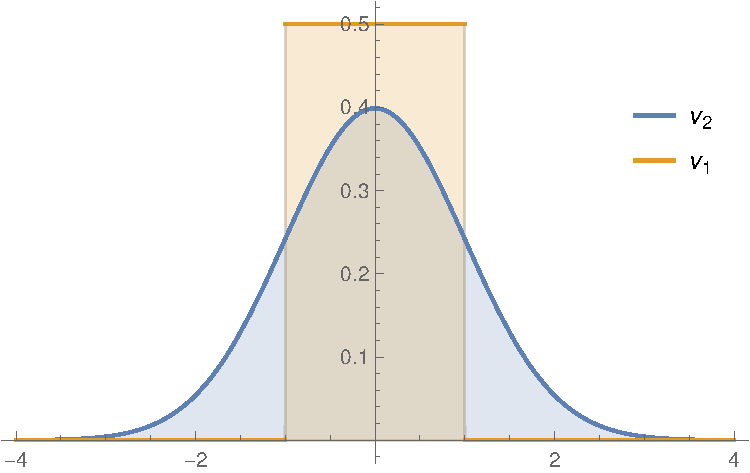
\includegraphics[height=.5\linewidth]{Chapters/OPT_line.pdf}
			\caption{Densities of $\nu_1$ and $\nu_2$}
		\end{minipage}
		\begin{minipage}{.49\textwidth}
			\centering
			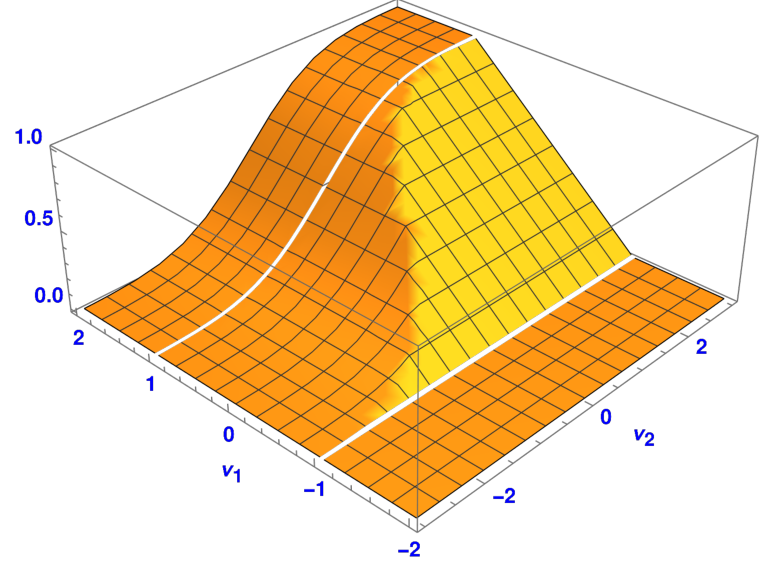
\includegraphics[height=.5\linewidth]{Chapters/cdf_line.pdf}
			\caption{CDF of optimal coupling}
		\end{minipage}
	\end{figure}
	We also draw the cumulative distribution function
	of optimal coupling between $\nu_1$ and $\nu_2$
	by \cite[Theorem 2.18]{villani2003topics}.
	By McCann's displacement interpolation (\cite[Section 5.1.3]{villani2003topics}),
	$\mu =[\frac{1}{2} \operatorname{Id} + \frac{1}{2} \nabla \psi]_{\#} \nu_1$ is the barycenter of $\mathbb{P}$.
	Then the support of $\mu$ could not be compact,
	otherwise the image of transference map is contained
	in a compact set for $\nu_1$ almost everywhere.
\end{rmk}
